###\section{Finanzmathematik}

\subsection{Leitgedanken der Finanzmathematik}
\begin{frame}{Leitgedanken - Finanzmathematik}
	\begin{bemerkung}[Leitgedanken]
	\begin{enumerate}
	\item Der Wert einer Zahlung ist \textbf{abhängig vom Zeitpunkt}, zu dem diese zu leisten ist.
	\item Es gilt stets das \textbf{Äquivalenzprinzip}.
	\item Das Gerüst der klassischen Finanzmathematik wird aus \textbf{ganz wenigen Formeln} gebildet.
	\item In der klassischen Finanzmathematik gibt es einfache, mittelschwere und relativ kompliziert zu lösende Probleme. Die größte Schwierigkeit ist in der Regel die \textbf{Modellierung}.
	\item Ein \textbf{grafisches Schema} bringt fast immer Klarheit.
	\item Das wichtigste Konzept ist das der \textbf{Rendite}, auch \textbf{Effektiv- oder Realzins} genannt.
	\item Die klassische Finanzmathematik läßt sich klar umreißen. Das wichtigste Konzept ist das des \textbf{Zinssatzes}.
	\end{enumerate}
	\end{bemerkung}
\end{frame}

\begin{frame}{Begriffe}
	\begin{itemize}
		\item[\textbf{Kapital}] Geldbetrag, der angelegt bzw. jemand anderem überlassen wird.
		\item[\textbf{Laufzeit}] Dauer der Überlassung/Anlage
		\item[\textbf{Zinsen}] Vergütung für die Kapitalüberlassung innerhalb einer Zinsperiode
		\item[\textbf{Zinsperiode}] der vereinbarten Verzinsung zugrunde liegender Zeitrahmen; meist ein Jahr, oftmals kürzer (Monat, Quartal, Halbjahr), selten länger
		\item[\textbf{Zinssatz}] Zinsbetrag in Geldeinheiten (GE), der für ein Kapital von 100 GE in einer Zinsperiode zu zahlen ist; auch \textbf{Zinsfuß} genannt.
		\item[\textbf{Zeitwert}] der von der Zeit abhängige Wert des Kapitals
	\end{itemize}
\end{frame}

\begin{frame}{Notation}
	\begin{bemerkung}
		Folgende Notation wird (in der Regel) im folgenden benutzt:
		\begin{itemize}
			\item Kapital: $K_{t}$ für das Kapital zum Zeitpunkt $t$
			\item Zinssatz: $i = \frac{p}{100}$ wobei $p$ der Zinssatz/Zinsfuß in Prozent ist.
			\item Aufzinsungsfaktor: $q = \left( 1+i \right) = \left(1 + \frac{p}{100}\right) $
			\item Zinsen: $Z_{t}$ Zinsen für den Zeitraum $t$.
		\end{itemize}
		\begin{center}
		Damit gelten folgende Zusammenhänge:
		\begin{tabular}{|c||c|c|c|}
				\hline \rule[-2ex]{0pt}{5.5ex}  & $p$ & $i$ & $q$ \\ 
				\hline \hline \rule[-2ex]{0pt}{5.5ex} $p$ & $p$ & $100 i$ & $100(q-1)$ \\ 
				\hline \rule[-2ex]{0pt}{5.5ex} $i$ & $\frac{p}{100}$ & $i$ & $q-1$ \\ 
				\hline \rule[-2ex]{0pt}{5.5ex} $q$ & $1+\frac{p}{100}$ & $1+i$ & $q$ \\ 
				\hline 
			\end{tabular}
		\end{center}
	\end{bemerkung}
\end{frame}

\subsection{Lineare Verzinsung}

\begin{frame}{Lineare Verzinsung}
	\begin{definition}
		\textbf{Zinsformel:} Zinsen hängen proportional vom Kapital $K$, der Laufzeit $t$ und dem Zinssatz $i$ ab:
		\[
			Z_{t} = K \cdot i \cdot t
		\]
	\end{definition}
	\begin{bemerkung}
		In Deutschland wird meist das Jahr zu 360 Tagen und der Monat zu 30 Zinstagen gerechnet. Daher kann man meist $t = \frac{T}{360}$ setzen, wobei $T$ die Anzahl an Tagen ist.
		\[
		Z_{T} = K \cdot i \cdot \frac{T}{360}
		\]
	\end{bemerkung}
\end{frame}

\begin{frame}{Beispiele}
	\begin{example}
		Welche Zinsen fallen an, wenn ein Kapital von 3500 € vom 3. März bis zum 18. August eines Jahres bei einem Zinssatz von 3.25 \% p.a. angelegt wird?	 
		
		\textbf{Antwort:} Da $165=27+30+30+30+30+18$ Zinstage zugrunde zu legen sind, ergibt sich aus der Zinsformel
		\[
		Z_{165} = 3500\mbox{ \euro} \cdot \frac{3.25}{100} \frac{165}{360} = 52.135416667 \mbox{ €} \approx 52.14 \mbox{ \euro}
		\] 
	\end{example}
	\begin{example}
		Wie hoch ist ein Kredit, für den in einem halben Jahr bei 8 \% Jahreszinsen 657.44 € Zinsen zu zahlen sind?
		
		\textbf{Antwort:} Durch Umstellen der Zinsformel ermittelt man:
		\[
		K=Z_{T} \frac{100}{p} \frac{360}{T} = 657.44 \mbox{ €} \cdot \frac{100}{8} \frac{360}{180} = 16 436 \mbox{ €}
		\]
	\end{example}
\end{frame}

\begin{frame}{Beispiele}
	\begin{example}
		Ein Wertpapier über 5000 €, das mit einem Kupon (Nominalzins) von 6.25 \% ausgestattet ist, wurde einige Zeit nach dem Emissionsdatum erworben. Es sind Stückzinsen in Höhe von 36.46 € zu zahlen. Wieviele Zinstage wurden dabei berechnet?
		
		\textbf{Antwort:} Umstellen der Zinsformel führt auf
		\[
			T = \frac{Z_{T} \cdot 100 \cdot 360}{K \cdot p} = \frac{36.46 \cdot 100 \cdot 360}{5000 \cdot 6.25} = 42 \mbox{ (Tage)}
		\] 
	\end{example}
\end{frame}

\begin{frame}{Zeitwert}
	\begin{definition}	
		Da sich das Kapital $K_{t}$ zum Zeitpunkt $t$ aus dem Anfangskapital $K_{0}$ zuzüglich der im Zeitraum $t$ angefallenen Zinsen $Z_{t}$ ergibt, also 
		\[
			K_{t} = K_{0} + Z_{t}
		\]
		gilt, folgt aus der Zinsformel eine sehr wichtige Formel der Finanzmathematik, die \textbf{Endwertformel bei linearer Verzinsung}
		\[
			K_{t} = K_{0} + Z_{t} = K_{0} + K_{0} \cdot i \cdot t = K_{0} \left( 1 + i \cdot t \right) = K_{0} \left( 1 + \frac{p}{100} \cdot t \right)
		\]
	\end{definition}
	\begin{bemerkung}
		Man kann durch Umstellen der Endwertformel auch den \textbf{Barwert} $K_{0}$ einer zukünftigen Zahlung $K_{t}$ berechnen
		\[
			K_{0} = \frac{K_{t}}{1+i \cdot t}
		\]
	\end{bemerkung}
\end{frame}

\begin{frame}{Beispiele}
	\begin{example}
		In einem halben Jahr ist eine Forderung von 8000 € fällig. Wie viel ist bei einer Sofortzahlung zu leisten, wenn mit einem kalkulatorischen Zins von i= 5 \% gerechnet wird?
		
		\textbf{Antwort:} Aus der Barwertformel ergibt sich
		\[
			K_{0} = \frac{8000}{1+0.05 \cdot \frac{1}{2}} \mbox{ €} = 7804.88 \mbox{ €}
		\]
	\end{example}
\end{frame}

\begin{frame}{Äquivalenzprinzip und Barwert}
	\begin{bemerkung}
		Das \textbf{Äquivalenzprinzip} nutzt man in der Finanzmathematik meist in der Form eines \textbf{Barwert-Vergleichs}, indem die Barwerte von Zahlungen, die zu verschiedenen Zeitpunkten geleistet werden, berechnet werden. 
	\end{bemerkung}
\end{frame}
\begin{frame}{Beispiel - Äquivalenzprinzip und Barwert}
	\footnotesize{
		\begin{example}
		Beim Verkauf einer Maschine werden dem Käufer zwei Angebote gemacht: Entweder 9000 € in 30 Tagen oder 9085 € in 90 Tagen. Welches Angebot ist günstiger, wenn jährlich mit 6 \% bzw. mit 3 \% verzinst wird? Bei welchem Zinssatz ergibt sich Gleichheit?
		
		\textbf{Antwort:}
		Bei einer Verzinsung von 6 \% ergeben sich folgende Barwerte:
		\[
			K_{0}^{30} = \frac{9000}{1+0.06 \cdot \frac{30}{360}} = 8955.22 \qquad 			K_{0}^{90} = \frac{9085}{1+0.06 \cdot \frac{90}{360}} = 8950.74  
		\] 
		Das zweite Angebot ist also bei 6 \% günstiger.
		
		Bei einer Verzinsung von 3 \% ergeben sich folgende Barwerte:
		\[
		K_{0}^{30} = \frac{9000}{1+0.03 \cdot \frac{30}{360}} = 8977.55 \qquad 			K_{0}^{90} = \frac{9085}{1+0.03 \cdot \frac{90}{360}} = 9017.37  
		\] 
		Das erste Angebot ist also bei 3 \% günstiger.

		Gleichwertigkeit beider Angebote führt auf die Gleichung 
		\[
		\frac{9000}{1+i \cdot \frac{30}{360}} = \frac{9085}{1+i \cdot \frac{90}{360}} \Leftrightarrow 9000 \cdot \left( 1 + i \frac{1}{4} \right) = 9085 \left( 1 + i \frac{1}{12} \right) 	
		\]
		Daraus folgt $i = 0.0569 = 5.69 \%$ 
	\end{example}}
\end{frame}

\begin{frame}{Berechnung von Zinssatz und Laufzeit}
	\begin{bemerkung}
		Man kann aus der Endwertformel bei linearer Verzinsung sowohl den Zinssatz als auch die Laufzeit berechnen:
		\[
		i = \frac{1}{t} \left( \frac{K_{t}}{K_{0}} - 1\right) \qquad t = \frac{1}{i} \left( \frac{K_{t}}{K_{0}} - 1\right)
		\]
	\end{bemerkung}
	\begin{example}
		In welcher Zeit wächst eine Spareinlage von 1200 € bei 2.8 \% jährlicher Verzinsung auf 1225.20 € an?
		
		\textbf{Antwort: } 
		\[
		t = \frac{1}{0.028} \left( \frac{1225.20}{1200} - 1 \right) = 0.75 = \frac{3}{4}
		\]
	\end{example}
\end{frame}

\subsection{Mehrfache konstante Zahlungen}

\begin{frame}{Mehrfache konstante Zahlung - vorschüssig}
	\begin{example}
	\textbf{Frage: }Welcher Endbetrag ergibt sich am Ende eines Jahres, wenn monatlich am Anfang eines Monats (\textbf{vorschüssig}) ein stets gleichbleibender Betrag $r$ bei einem Zinssatz von $i$ angelegt wird?
	
	\textbf{Antwort:} Die erste Zahlung wird 12 Monate lang verzinst, wächst also mit dem Faktor $1+i\frac{12}{12}$, die zweite nur 11 Monate, wächst also mit dem Faktor $1+i\frac{11}{12}$ usw. Alle Zahlungen gemeinsam ergeben damit die Gesamtsumme\footnote{Da kommt die Gaußsche Summenformel vor! Erinnern Sie sich?} 
	\begin{align*}
		R & = r \left( 1 + i \frac{12}{12} + 1 + i \frac{11}{12} + 1 + i \frac{10}{12} +\cdots + 1 + i \frac{1}{12} \right) \\
		& = r \left( 12 + \frac{i}{12} \left( 12 + 11 + 10 + \cdots + 1 \right) \right) \\
		& = r \left( 12 + \frac{i}{12}  \frac{13 \cdot 12}{2}\right) = r \left( 12 + 6.5 i \right)
	\end{align*}
	\end{example}	
\end{frame}

\begin{frame}{Mehrfache konstante Zahlung - nachschüssig}
	\begin{example}
		\textbf{Frage: }Welcher Endbetrag ergibt sich am Ende eines Jahres, wenn monatlich am Ende eines Monats (\textbf{nachschüssig}) ein stets gleichbleibender Betrag $r$ bei einem Zinssatz von $i$ angelegt wird?
		
		\textbf{Antwort:} Die erste Zahlung wird 11 Monate lang verzinst, wächst also mit dem Faktor $1+i\frac{11}{12}$, die zweite nur 10 Monate, wächst also mit dem Faktor $1+i\frac{10}{12}$ usw. Alle Zahlungen gemeinsam ergeben damit die Gesamtsumme
		\begin{align*}
		R & = r \left( 1 + i \frac{11}{12} + 1 + i \frac{10}{12} + 1 + i \frac{9}{12} +\cdots + 1 + i \frac{0}{12} \right) \\
		& = r \left( 12 + \frac{i}{12} \left( 11 + 10 + 9 + \cdots + 1 \right) \right) \\
		& = r \left( 12 + \frac{i}{12}  \frac{12 \cdot 11}{2}\right) = r \left( 12 + 5.5 i \right)
		\end{align*}
	\end{example}	
\end{frame}


\begin{frame}{Mehrfache konstante Zahlungen - beliebige Zahlungsfrequenz - Jahresersatzrate}
	\footnotesize{
	\begin{bemerkung}
		Wird allgemein ein Jahr in $m$ kürzere Perioden der Länge $\frac{1}{m}$ aufgeteilt und zu jedem Zeitpunkt $\frac{k}{m}$ mit $k=0, 1, \ldots, m-1$, also vorschüssig eine Zahlung $r$ geleistet, so ergibt sich am Ende des Jahres ein Betrag von
		\[
		R^{\text{vor}} = r \left( \sum_{k=0}^{m-1} 1 + i \cdot \frac{k+1}{m} \right) = r \left( \sum_{k=1}^{m} 1 + i \cdot \frac{k}{m} \right) = r \left( m + \frac{m+1}{2} \underset{=i}{\underbrace{\frac{p}{100}}} \right)
		\] 
		Werden die Zahlungen zu den Zeitpunkten $\frac{k}{m}$ mit $k=1, 2, \ldots, m$, also nachschüssig geleistet, so gilt
		\[
		R^{\text{nach}} = r \left( \sum_{k=0}^{m-1} 1 + i \cdot \frac{k}{m} \right) = r \left( m + \frac{m-1}{2} \underset{=i}{\underbrace{\frac{p}{100}}} \right)
		\]
		Die Beträge $R^{^\text{vor}}$ und $R^{^\text{nach}}$ heißen \textbf{vorschüssige} bzw. \textbf{nachschüssige Jahresersatzrate}. Sie geben den Wert einer jährlichen Zahlung an, die den m vor- bzw. nachschüssigen $\frac{1}{m}$-periodischen Zahlungen r äquivalent ist.
	\end{bemerkung}}
\end{frame}

\begin{frame}{Beispiel Jahresersatzrate}
	\begin{example}
	Ein Student schließt einen Sparplan über die Laufzeit von einem Jahr mit folgenden Konditionen ab: Einzahlungen von 75 € jeweils zu Monatsbeginn (Monatsende), Verzinsung mit 4 \% p.a., Bonus am Jahresende in Höhe von 1 \% aller Einzahlungen. Über welche Summe kann der Student am Ende des Jahres verfügen?
	
	\textbf{Antwort: } In der Formel für die Jahresersatzrate ist hier $m=12$ und damit für den Endwert $E$ der Zahlungen ohne Bonus
	\begin{align*}
		E^{\text{vor}} &  = 75 \cdot \left( 12+6.5 \cdot 0.04 \right) = 919.50 \text{\tiny{ bei vorschüssiger Zahlung am Monatsanfang}} \\
		E^{\text{nach}} &  = 75 \cdot \left( 12+5.5 \cdot 0.04 \right) = 916.50 \text{\tiny{ bei nachschüssiger Zahlung am Monatsende}}
	\end{align*}
	Die Bonuszahlung beträgt $12 \cdot 75 \cdot 0.01 = 9.00$, woraus sich die Gesamtbeträge
		\begin{align*}
		E^{\text{vor}}_{\text{gesamt}} & = 919.50 + 9.00 = 928.50 \text{\tiny{ bei vorschüssiger Zahlung am Monatsanfang}} \\
		E^{\text{nach}}_{\text{gesamt}} & = 916.50 + 9.00 = 925.50 \text{\tiny{ bei nachschüssiger Zahlung am Monatsende}}
		\end{align*}
\end{example}		
\end{frame}

\begin{frame}{Skontoabzug}
	\begin{bemerkung}
		Bei sofortiger Bezahlung von Waren bzw. Dienstleistungen vor dem Fälligkeitstermin der Rechnung wird oft ein Nachlass (\textbf{Skonto}) gewährt. Bezeichnet $s$ die Größe des Skontos, $R$ den Rechnungsbetrag und $T$ die Differenztage der Zahlungsziele, so zahlt man also bei Sofortbezahlung nur den Betrag
		\[
			\left(1-s\right) R
		\] 
		Den zugehörigen \textbf{Effektivzinssatz} $i_{\text{eff}}$ kann man dann mit Hilfe der Barwertformel berechnen
		\[
			\left(1-s\right) R = \frac{R}{1+i_{\text{eff}}\cdot\frac{T}{360}} \qquad \Leftrightarrow \qquad i = \frac{s}{1-s} \cdot \frac{360}{T}
		\]
	\end{bemerkung}
\end{frame}

\begin{frame}{Beispiel Skonto - Effektivzins}
	\begin{example}
		Auf einer Handwerkerrechnung über die Summe $R$ lauten die Zahlungsbedingungen:
		 \glqq Bei Zahlung innerhalb von 10 Tagen gewähren wir 2 \% Skonto. Zahlung innerhalb von 30 Tagen ohne Abzug. \grqq 
		 
		 Für den Effektivzins ergibt sich hier:
		 \[
			 i_{\text{eff}} = \frac{0.02}{0.98} \cdot \frac{360}{20} = 0,3673469388
		 \]
		 Man sollte also von der Möglichkeit des Skontos Gebrauch machen, das dies einer Verzinsung des Kapitals mit 36.73 \% entspricht.
	\end{example}
\end{frame}

\begin{frame}{Beispiele zum Selberrechnen}
{\small 	\begin{example}
		Ein Schuldner überweist seinem Gläubiger am 15.12. Verzugszinsen in Höhe von 821,37 €. für einen seit dem 28.04. desselben Jahres ausstehenden Rechnungsbetrag in Höhe von 10600 €. Welchem nachschüssigen Zinssatz p.a. entspricht diese Zinszahlung?
	\end{example}
	\begin{example}
		Sie leihen sich 9000 € am 15.03. und zahlen 10000 € am 11.11. zurück. Zu welchem Effektivzinssatz erhielten sie den Kredit?
	\end{example}
	\begin{example}
		Wann müsste eine Zahlung in Höhe von 20000 € fällig sein, damit sie äquivalent ist zu einer am 5.5.2016 fälligen Zahlung in Höhe von 19500 € bzw. 21.000 € bei einem Zinssatz von 12 \% p.a. 	
	\end{example}		
}\end{frame}

%%% Selber-Rechnen-Lösungen: ANFANG
\begin{frame}{Beispiele zum Selberrechnen}
	\begin{example}
		Ein Schuldner überweist seinem Gläubiger am 15.12. Verzugszinsen in Höhe von 821,37 €. für einen seit dem 28.04. desselben Jahres ausstehenden Rechnungsbetrag in Höhe von 10600 €. Welchem nachschüssigen Zinssatz p.a. entspricht diese Zinszahlung?
		
		\textbf{Lösung:} Die Anzahl der Zinstage vom 28.04. bis zum 15.12. ist $2 + 7 \times 30 + 15 = 227$. 
		Umstellen der Formel für die lineare Verzinsung
		\[
		Z = K \cdot i \cdot t = K \cdot i \cdot \frac{T}{360}
		\] 
		nach i ergibt
		\[
		i = \frac{Z}{K \cdot \frac{T}{360}} = \frac{360 \cdot Z}{K \cdot T} = \frac{360 \cdot 821.37}{10600 \cdot 227} = 0.12288...
		\] 
		also ca. 12,3 \% .
	\end{example}
\end{frame}

\begin{frame}{Beispiele zum Selberrechnen}
\footnotesize{		\begin{example}
			Sie leihen sich 9000 € am 15.03. und zahlen 10000 € am 11.11. zurück. Zu welchem Effektivzinssatz erhielten sie den Kredit?
			
			\textbf{Lösung:} Hier kann man zwei Lösungwege einschlagen:
			\begin{itemize}
				\item \textbf{Lösung A:} Der Barwert von 10000 €, fällig am 11.11., berechnet für den 15.03. soll 9000 € betragen. Mit der Barwertformel
				\[
					K_{0} = \frac{K_{T}}{\left(1 + i \frac{T}{360}\right)} \Leftrightarrow i = \left(\frac{K_{T}}{K_{0}} - 1 \right) \frac{360}{T}  
				\] 
				und $T =  15 + 7 \cdot 30 + 11 = 236$ ergibt sich:
				\[
				i = \frac{360}{236} \cdot \left( \frac{10000}{9000} - 1  \right) = 0,1694915254
				\]
				also ca. 16,95 \% .
				\item \textbf{Lösung B:} Für die 9000 € sind am 11.11. neben der Rückzahlung auch 1000 €  =10000 € - 9000 € Zinsen fällig. Umstellen der Zinsformel ergibt
				\[
				i = \frac{Z}{K \cdot \frac{T}{360}} = \frac{360 \cdot Z}{K \cdot T} = \frac{360 \cdot 1000}{9000 \cdot 236} = 0,1694915254
				\] 		
			\end{itemize} 
		\end{example}	}	
\end{frame}

\begin{frame}{Beispiele zum Selberrechnen}
\small{	\begin{example}
		Wann müsste eine Zahlung in Höhe von 20000 € fällig sein, damit sie äquivalent ist zu einer am 9.5.2016 fälligen Zahlung in Höhe von 19500 € bzw. 21.000 € bei einem Zinssatz von 12 \% p.a. 
		
		\textbf{Lösung:} 
		\begin{itemize}
 			\item \textbf{Zahlung 19500 €:} Die Anzahl der Zinstage ist hier gesucht. Umstellen der Barwertformel nach $T$ ergibt:
 			\[
 			T = \left( \frac{K_{T}}{K{0}} - 1 \right) \frac{360}{i} = \frac{360}{0.12} \left( \frac{20000}{19500} - 1\right) = 76,9230768
 			\]
 			also etwa 77 Tage nach dem 9.5.2016, also am 26.07.2016.
			
			\item \textbf{Zahlung 21000 €:} Die Anzahl der Zinstage ist hier gesucht. Umstellen der Barwertformel nach $T$ ergibt:
			\[
			T = \left( \frac{K_{T}}{K{0}} - 1 \right) \frac{360}{i} = \frac{360}{0.12} \left( \frac{20000}{21000} - 1\right) = -142,8571428
 			\]
 			also etwa 143 Tage vor dem 9.5.2016, also am 16.12.2015.		
		\end{itemize} 

	\end{example}}		
\end{frame}
%%% Selber-Rechnen-Lösungen: ENDE


\begin{frame}{Ratenzahlungen}
	\begin{example}
		Oft besteht die Möglichkeit, Zahlungen entweder direkt oder als Ratenzahlungen mit gewissen Aufschlägen zu leisten.
		
		Beispielsweise können Autoversicherungen entweder am Jahresanfang oder in zwei Raten mit jeweils 5 \% Aufschlag zum Jahresbeginn und nach einem halben Jahr gezahlt werden.
		
		Für den Effektivzins gilt dann nach dem Äquivalenzprinzip:
		\[
		R =  \frac{1.05 \cdot R}{2} +  \frac{1.05 \cdot R}{2} \frac{1}{1+\frac{i}{2}}
		\]
		Nach Kürzen von $R$ und Auflösen nach dem Zinssatz $i$ ergibt sich ein Wert von $i=0.210526$, also 21.0526 \%. Da dieser Zinssatz relativ hoch ist, sollte man sich für die Bezahlung am Jahresanfang entscheiden.
	\end{example}
\end{frame}

\subsection{Tageszählweisen - Day Count Conventions}
\begin{frame}{Tageszählweisen - Day Count Conventions}
	\begin{bemerkung}
		Bisher wurde in den verschiedenen Formeln die Zeit $t$ einfach als Teil der Zinsperiode betrachtet. In der Praxis ist aber gar nicht immer so klar, wie diese Zahl berechnet werden soll, denn bei der Berechnung der Laufzeit
		\[
		t = \frac{\text{Zinstage (Laufzeittage) }}{\text{Tagebasis (Jahreslänge in Tagen)}}
		\]
		als Teil des Jahres gibt es verschiedene Zinsmethoden. Wir haben bisher die sogenannte \textbf{Bond-Methode} benutzt, in der Monate 30 Tage haben und das Jahr 360 Tage.
	\end{bemerkung}
\end{frame}

\begin{frame}{Tageszählweisen - Day Count Conventions}
	\scriptsize{\begin{bemerkung}
		Es gibt weltweit noch einige andere Tageszählweisen / Day Count Conventions:
		\begin{tabular}{|p{1.3cm}p{1.1cm}p{1.3cm}p{0.9cm}p{3.4cm}|}
			\hline \rule[-2ex]{0pt}{5.5ex} Methode & Name & Anzahl Zinstage/Monat & Tagebasis (Jahr) & Anwendung \\ 
			\hline \hline \rule[-2ex]{0pt}{5.5ex} 30E/360 & Bond-Methode & 30 & 360 & in Deutschland für Sparbücher, Wertpapiere und Termingelder \\ 
			\hline \rule[-2ex]{0pt}{5.5ex} 30/360 & Bond-Methode & 30 & 360 & viele Computerprogramme und Taschenrechner arbeiten nach dieser Methode \\ 
			\hline \rule[-2ex]{0pt}{5.5ex} act/360 & Eurozins-Methode & kalendergenau & 360 & am Euromarkt für das alle Währungen, in Deutschland z.B. für Floating Rate Notes \\ 
			\hline \rule[-2ex]{0pt}{5.5ex} act/365 & Englische Methode & kalendergenau & 365 & z.B. für die Währungen GBP und BEF, in Deutschland bei Geldmarktpapieren \\ 
			\hline \rule[-2ex]{0pt}{5.5ex} act/act &  & kalendergenau & 365/366 &  \\ 
			\hline 
		\end{tabular} 
	\end{bemerkung}}
\end{frame}

\begin{frame}{Tageszählweisen - Besonderheiten}
	\begin{bemerkung}
		\begin{itemize}
			\item \textbf{30E/360-Methode} Fällt ein Zinstermin auf den 31. Tag eines Monats, so wird er auf den 30. gelegt. Auch der Februar wird mit 30 Tagen veranschlagt, es sei denn, das Geschäft endet am 28./29. Februar, dann umfasst er 28/29 Tage.
			\item \textbf{30/360-Methode} Analog zur 30E/360-Methode mit folgendem Unterschied: Endet ein Geschäft an einem 31. und hat es nicht am 30. oder 31. eines Monats begonnen, so wird im Endmonat mit 31 Zinstagen gerechnet.
			\item \textbf{act/act-Methode} Für angebrochene Jahre werden die Laufzeittage zeitabhängig gewichtet berechnet. Erstreckt sich der Zeitraum zusätzlich über volle Jahre, so werden die entsprechenden Jahre zur Laufzeit addiert. 
		\end{itemize}
	\end{bemerkung}
\end{frame}

\begin{frame}{Tageszählweisen - Besonderheiten}
	\begin{bemerkung}
		\textbf{Konventionen bei Feiertagen (Nicht-Bankarbeitstagen)}
		
		Ist ein Fälligkeitstermin kein Bankarbeitstag, wird unterschiedlich verfahren:
		
		\begin{itemize}
			\item \textbf{Following:} Es wird der nächste Bankarbeitstag genommen.
			\item \textbf{Modified Following:} Es wird der nächste Bankarbeitstag genommen, falls dieser im gleichen Monat liegt, ansonsten der vorhergehende Bankarbeitstag
			\item \textbf{Preceding:} Es wird der vorhergehende Bankarbeitstag genommen.
			\item \textbf{Modified Preceding:} Es wird der vorhergehende Bankarbeitstag genommen, falls dieser im gleichen Monat liegt, ansonsten der folgende Bankarbeitstag	
		\end{itemize}	
	\end{bemerkung}	
\end{frame}

\subsection{Zinseszinsrechnung}
\begin{frame}{Zinseszinsrechnung}
	\begin{bemerkung}
		Wird ein Kapital über mehrere Zinsperioden (Jahre) hinweg angelegt und werden dabei jeweils am Jahresende fälligen Zinsen angesammelt und in den folgenden Jahren mitverzinst, entstehen \textbf{Zinseszinsen}.
		\begin{align*}
		K_{1} & = K_{0} \left( 1 + i \right) = K_{0} q \text{ mit } q= (1+i) \\
		K_{2} & = K_{1} \left( 1 + i \right) = K_{1} q = K_{0} q \cdot q = K_{0} q^2 \\
		K_{3} & = K_{2} \left( 1 + i \right) = K_{2} q = K_{0} q^2 \cdot q= K_{0} q^3  \\
		K_{n} & = K_{0} q^n
		\end{align*}
		Die letztere Formel nennt sich \textbf{Endwertformel bei geometrischer Verzinsung} oder \textbf{Leibnizsche Zinseszinsformel}. 
	\end{bemerkung}
\end{frame}

\begin{frame}{Beispiel Zinseszins}
 	\begin{example}
		Für einen Sparbrief über 4000 €, der über fünf Jahre hinweg unter Zinsansammlung konstant mit 6 \% verzinst wird erhält man am Ende des 5. Jahres
		\[
		K_{5} = K_{0} \left(1 + 0.06 \right)^5 = 4000 \text{€} \cdot \left( 1.06 \right)^5 = 5352.60 \text{€}
		\]
	\end{example}
	\begin{bemerkung}
		$K_{5}$ kann man hier auch als Endwert bezeichnen; $K_{0}$ nennt man (auch hier) Barwert (in diesem Falle der Barwert einer Zahlung in Höhe von $K_{5}$, die in fünf Jahren stattfindet). Die Formel für den Barwert ist dann:
		\[
		K_{0} = \frac{K_{n}}{q^{n}}
		\]
	\end{bemerkung}
\end{frame}

\begin{frame}{Unterjährige Verzinsung mit Zinseszins}
	\begin{bemerkung}
		Werden Zinsen auch unterjährig für Zinsperioden gutgeschrieben, die kleiner als ein Jahr sind, also beispielsweise nach $\frac{1}{m}$ Jahren, also $m$-mal im Jahr, so gilt analog zur Endwertformel
		\begin{align*}
		K_{1} & = K_{0} \left( 1 + \frac{i}{m}\right) = K_{0} q \text{ mit } q= (1+\frac{i}{m}) \\
		K_{2} & = K_{1} \left( 1 + \frac{i}{m} \right) = K_{1} q = K_{0} q \cdot q = K_{0} q^2 \\
		K_{3} & = K_{2} \left( 1 + i \right) = K_{2} q = K_{0} q^2 \cdot q= K_{0} q^3  \\
		K_{n\cdot m} & = K_{0} q^{n \cdot m} = K_{0} \left( 1+ \frac{i}{m} \right)^{n \cdot m}
		\end{align*}
		Hier bezeichnet der Index $i$ am Kapital $K_{i}$ die Anzahl der Zinsperioden; da es $m$ Zinsperioden pro Jahr gibt, hat man nach $n$ Jahren $n \cdot m$ Zinsperioden verzinst. Dafür enthält der Aufzinsungsfaktor $q = \left( 1+ \frac{i}{m} \right)$ nur den $m$-ten Teil ($\frac{1}{m}$) der Zinsen p.a.
	\end{bemerkung}
\end{frame}

\begin{frame}{Bemerkung zur unterjährigen Verzinsung mit Zinseszins}
\small{	\begin{bemerkung}
		In der Formel für die unterjährige Verzinsung mit Zinseszins
		\[
		K_{n \text{ Jahre}} = K_{n \cdot m} = K_{0} \left(  1+ \frac{i}{m}\right)^{n \cdot m}
		\]
		könnte man die Anzahl $m$ der Zinsperioden pro Jahr beliebig groß wählen; die einzelnen Zinsperioden werden dann immer kürzer ($\frac{1}{m}$ Jahre). Betrachtet man dann den Grenzwert unendlich vieler Zinsperioden
		\[
		K_{n \text{ Jahre}} = \lim_{m \to \infty} K_{0} \left(  1+ \frac{i}{m}\right)^{n \cdot m} = K_{0} \lim_{m \to \infty} \left(  1+ \frac{i}{m}\right)^{n \cdot m} = K_{0} e^{i \cdot n} 
		\]
		so ergibt sich die Formel für \textbf{exponentielle Verzinsung}, wobei $e$ die Basis des natürlichen Logarithmus $\ln$ ist.
	\end{bemerkung}}
\end{frame}

\begin{frame}{Abhängigkeit des Endwertes von der Zahl der Zinsperioden}
	\small{Bei einem Zinssatz von 10 \% ergibt sich folgende Abhängigkeit des Jahres-Endwertes von der Anzahl der Zinsperioden im Jahr:
	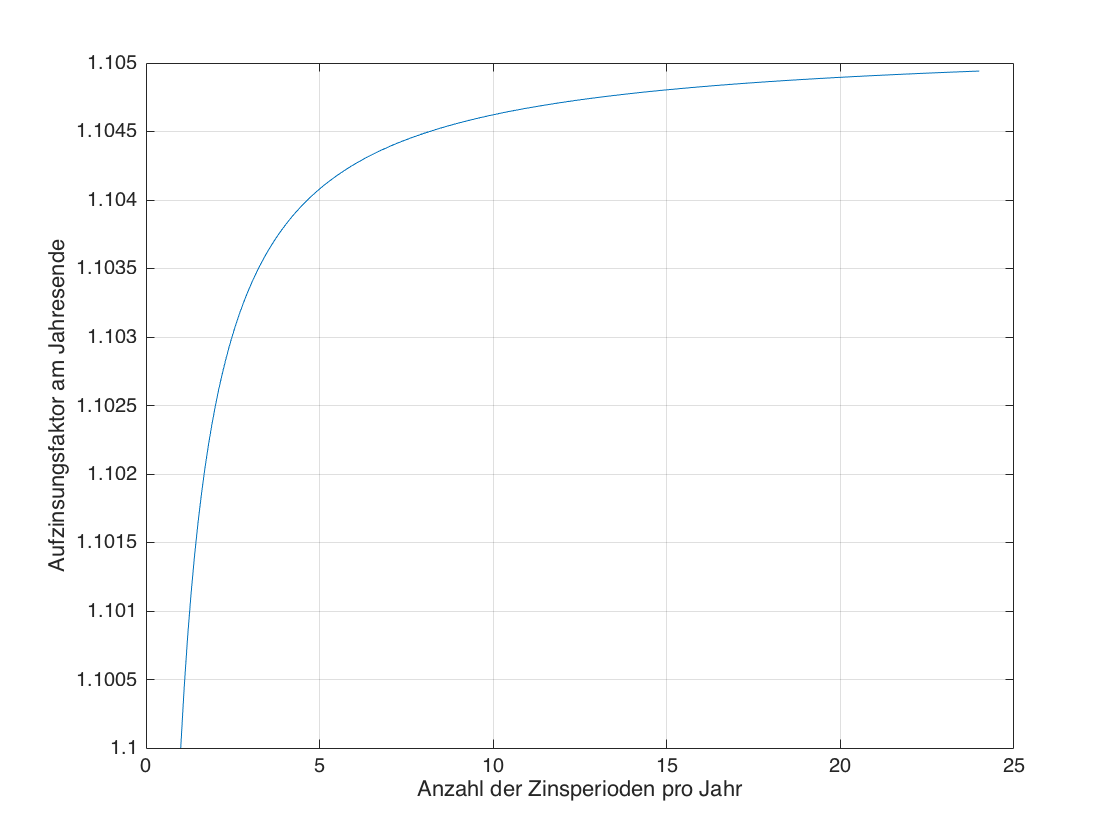
\includegraphics[width=9.5cm]{Matlab/exponentielleVerzinsung}}
\end{frame}

\begin{frame}{Effektiver Jahreszins}
\small{	\begin{bemerkung}
		Da der Endwert des Kapitals von der Anzahl der Zinsperioden (bei gleichem Zinssatz) abhängt, kann man sich fragen, was der äquivalente Zinssatz p.a. bei jährlicher Verzinsung wäre.
		
		Dazu vergleicht man den Endwert bei jährlicher Verzinsung mit einem Zinssatz $i_{\text{eff}}$ mit dem Endwert bei m-periodischer Verzinsung mit dem Zinssatz $i$:
		\begin{align*}
		K_{0} \left( 1+i_{\text{eff}} \right)^{n}  & = K_{0} \left( 1+\frac{i}{m} \right)^{n \cdot m} \\
		\Leftrightarrow i_{\text{eff}} & = \left( \left( 1+\frac{i}{m}  \right)^{m} -1 \right) 
		\end{align*}
	\end{bemerkung}
	\begin{bemerkung}
		Der \textbf{effektive Jahreszins} (auch \textbf{Rendite} genannt) $i_{\text{eff}}$ ergibt sich als Zinssatz, mit dem das Anfangskapital $K_{0}$ nachschüssig am Jahresende verzinst werden müsste, um denselben Endbetrag zu erzielen wie bei einer unterjährig m-mal mit Zinseszins verzinsten Anlageform.
	\end{bemerkung}}
\end{frame}

\begin{frame}{Effektivzins in Abhängigkeit von der Anzahl der Zinsperioden}
	\small{Bei einem Zinssatz von 10 \% ergibt sich folgende Abhängigkeit des Effektivzinses von der Anzahl der Zinsperioden im Jahr:
		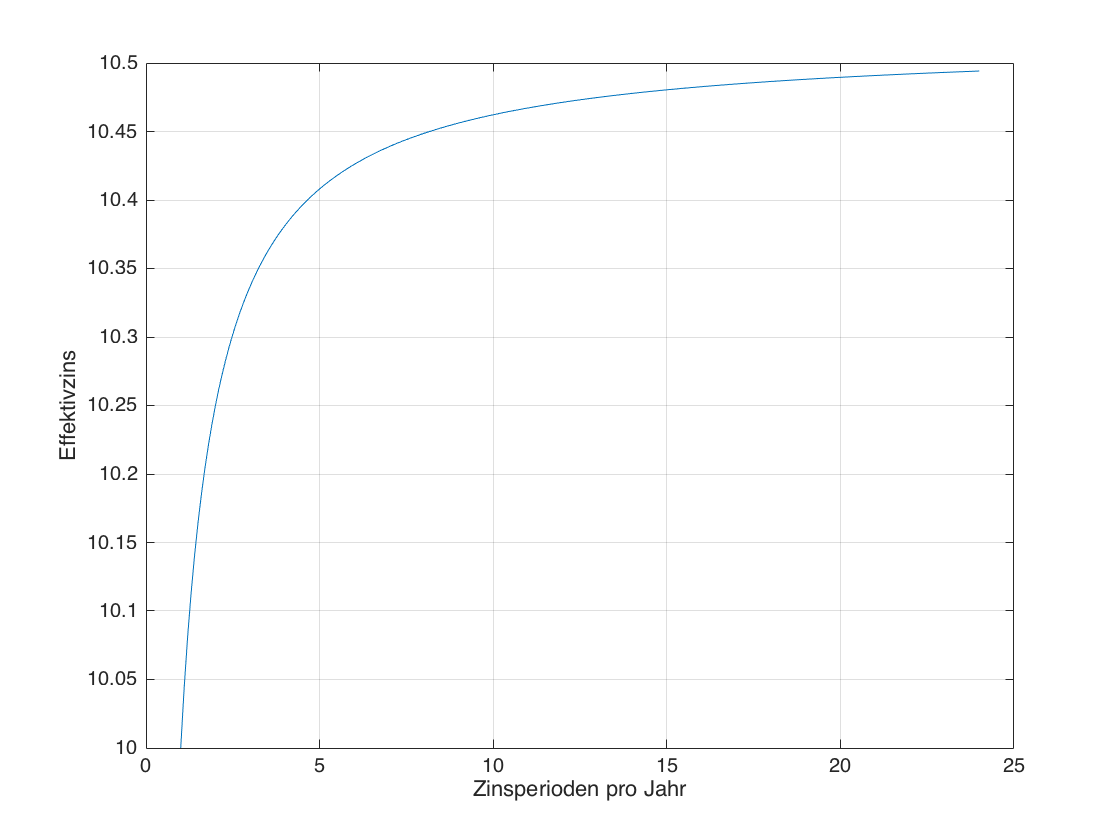
\includegraphics[width=9.5cm]{Matlab/effektivzins}		}
\end{frame}

\begin{frame}{Gemischte Verzinsung}
	\begin{bemerkung}
		Nur selten beginnt eine Anlage genau am Anfang einer Zinsperiode (z.B. bei jährlicher Verzinsung am Jahresanfang). Ebenso selten endet eine Anlage genau am Ende eines Zinsperiode (z.B. am Ende eines Jahres bei jährlicher Verzinsung),
		
		In der Regel verwendet mal also eine \textbf{gemischte Verzinsung}.
	\end{bemerkung}
	\small{\begin{example}
		Welchen Endwert hat eine Anlage von 10000 € vom 15. August 2015 zu einem Zinssatz von 12 \% am 16. März 2019?
		
		\textbf{Antwort:} Die erste Zinsperiode ist kein ganzes Jahr, sondern nur 135 Tage. Danach kommen 3 volle Jahre, danach nochmal 76 Tage, also:
		\[
		K_{\text{16. März 2019}} = \left( 1+0.12\cdot\frac{135}{360}  \right) \cdot \left( 1+0.12 \right)^{3} \cdot \left( 1+0.12\frac{76}{360} \right) \approx 15053.43
		\]
	\end{example}}
\end{frame}

\begin{frame}{Zinskurveneffekte}
\small{	\begin{bemerkung}
		Nur selten sind die Zinssätze, zu denen Geld angelegt oder geliehen werden kann, unabhängig vom Anlagezeitraum. 
		Eine \textbf{normale Zinskurve} zeigt vielmehr mit der Laufzeit der Anlage steigende Zinssätze.
		Zudem kann das Kapital im Laufe seines Anlagezeitraums unterschiedliche Zinssätze erfahren.
	\end{bemerkung}
	\begin{example}
		Ein Anfangskapital von 10000 € wird zunächst 2 Jahre lang mit 6 \% , danach 5 Jahre lang mit 7 \% und anschließend 3 Jahre lang mit 4 \% verzinst. 
		
		\textbf{Auf welchen Endwert ist das Kapital angewachsen und welchem Effektivzins entspricht die Anlage?}
		
		\textbf{Antwort:} 
		\[
		K = K_{0} \left( 1+0.06 \right)^{2} \cdot \left( 1+0.07 \right)^{5} \cdot \left( 1+0.04 \right)^{3} 
		\]
		Für den Effektivzins gilt:
		\[
		\left(1+i_{\text{eff}}\right)^{10} = \left( 1+0.06 \right)^{2} \cdot \left( 1+0.07 \right)^{5} \cdot \left( 1+0.04 \right)^{3}
 		\]
		
	\end{example}}
\end{frame}

\begin{frame}{Laufzeitberechnung}
	\begin{example}
		In welchem Zeitraum verdreitfacht sich ein Kapital bei einem Zinssatz (mit Zinseszins) von 5 \% p.a.?
		
		\textbf{Antwort:} Gesucht ist die Anzahl an Jahren $n$ in der Zinseszinsformel:
		\[
			K_{n} = 3 \cdot K_{0} = K_{0} \cdot \left( 1+0.05 \right)^{n}
		\]
		Diese Gleichung hat die Lösung
		\[
			n = \frac{\log 3}{\log 1.05} = 22,517085304
		\]
		Also verdreifacht sich das Kapital bei einem Zinssatz von 5\% in etwa 22,5 Jahren.
	\end{example}
\end{frame}

\begin{frame}{Zinseszinsformel}
{\footnotesize 	\begin{bemerkung}
		Falls man in der Zinseszinsformel mit den Aufzinsungsfaktoren rechnet, wird vieles einfacher:
		\begin{align*}
			K_{1} & = K_{0} \cdot (1+i) = K_{0} \cdot q \\
			K_{2} & = K_{1} \cdot (1+i) = K_{0} \cdot q^{2} \\
			K_{n} & = K_{0} \cdot (1+i)^{n} = K_{0} \cdot q^{n}
 		\end{align*}
 		Das gilt auch, wenn die Zinssätze verschieden sind:
		\begin{align*}
		K_{1} & = K_{0} \cdot (1+i_{1}) = K_{0} \cdot q_{1} \\
		K_{2} & = K_{1} \cdot (1+i_{2}) = K_{0} \cdot q_{1} \cdot q_{2} \\
		K_{n} & = K_{0} \cdot (1+i_{1}) \cdot (1+i_{2}) \cdot \ldots \cdot (1+i_{n}) = K_{0} \cdot q_{1} \cdot q_{2} \cdot q_{3} \cdot \ldots \cdot q_{n}
		\end{align*}
		Damit gilt für den Effektivzins:
		\begin{align*}
		K_{n} = K_{0} \underset{=: q_{\text{eff}}}{\underbrace{(1 + i_{\text{eff}})}}^{n} & = K_{0} q_{1} q_{2} \cdots q_{n} \\
		q_{\text{eff}}^{n} & = q_{1} q_{2} \cdots q_{n} \\
		q_{\text{eff}} & = \sqrt[n]{q_{1} q_{2} \cdots q_{n}}
		\end{align*}
		Der Effektivzins ist also über das \textbf{geometrische Mittel} der Aufzinsungsfaktoren zu berechnen.
	\end{bemerkung}
}\end{frame}

\begin{frame}{Beispiel - Rendite}
{\small 	\begin{example}
		Sie kaufen Bundesschatzbriefe vom Typ B (mit Zinseszins) im Nennwert von 10000 €, die folgende Verzinsung versprechen: 3.5 \% im 1. Jahr, 3.75 \% im 2. Jahr, 4 \% im 3. Jahr, 4.5 \% im 4. Jahr, 5 \% im 5. Jahr, 5.5 \% im 6. Jahr 6.5 \% im 7. Jahr.
		
		Welche Endsumme und welche Rendite erzielt diese Anlage, wenn man das Wertpapier über die vollen sieben Jahr hält?
		
		\textbf{Antwort:} Der Endwert berechnet sich
		\begin{align*}
		K_{7} & = K_{0} \cdot q_{1} \cdot q_{2} \cdots q_{7} \\ 
		& = 10000 \cdot 1.035 \cdot 1.0375 \cdot 1.04 \cdot 1.045 \cdot 1.05 \cdot 1.055 \cdot 1.065 \\ 
		& = 13767.96 \text{€}  
		\end{align*}
		Für den Effektivzins gilt:
		\begin{align*}
		\left( 1+ i_{\text{eff}} \right)^{7} & = q_{\text{eff}}^{7} & = 1.035 \cdot 1.0375 \cdot 1.04 \cdot 1.045 \cdot 1.05 \cdot 1.055 \cdot 1.065 \\
		\Leftrightarrow \left( 1 + i_{\text{eff}} \right) & = q_{\text{eff}} & = \sqrt[7]{1.035 \cdot 1.0375 \cdot 1.04 \cdot 1.045 \cdot 1.05 \cdot 1.055 \cdot 1.065}  \\
		\Leftrightarrow i_{\text{eff}} & & = q_{\text{eff}} - 1  = \sqrt[7]{1.376795543} -1 = 0.046739211
		\end{align*}
	\end{example}
}\end{frame}

\subsection{Rentenrechnung}
\begin{frame}{Rentenrechnung}
	\begin{definition}
		
	\end{definition}
\end{frame}

\begin{frame}{Endwert einer nachschüssigen Rente}
	\textbf{Frage}: Welchen Wert hat eine Rente mit der nachschüssigen (N) Rentenrate $R$, die über $n$ Jahre gezahlt wird, am Ende der Laufzeit?
	
	\footnotesize{
	\textbf{Antwort}: \begin{tabular}{|c|c|c|c|}
		\hline Jahr & nachschüssige Rate & verbleibender Zeitraum & Endwert der Rate \\ 
		\hline $1$ & $R$ & $n-1$ & $Rq^{n-1}$ \\ 
		\hline $2$ & $R$ & $n-2$ & $Rq^{n-2}$ \\ 
		\hline $3$ & $R$ & $n-3$ & $Rq^{n-3}$ \\ 
		\hline \vdots & \vdots & \vdots & \vdots \\ 
		\hline $n-2$ & $R$ & $2$ & $Rq^{2}$ \\ 
		\hline $n-1$ & $R$ & $1$ & $Rq$ \\ 
		\hline $n$ & $R$ & $0$ & $R$ \\ 
		\hline 
	\end{tabular}
	
	Damit ist
	\[
	R_{n}^{N} = R + Rq + Rq^{2} + R q^{3} + \ldots + Rq^{n-1} = \sum\limits_{i=1}^{n} Rq^{i-1} = R \sum\limits_{i=1}^{n} q^{i-1} = R \frac{q^{n}-1}{q-1}
	\] }
\end{frame}

\begin{frame}{Barwert einer nachschüssigen Rente}
	\textbf{Frage}: Welchen Barwert hat eine Rente mit der nachschüssigen (N) Rentenrate $R$, die über $n$ Jahre gezahlt wird, heute?
	
	\footnotesize{
		\textbf{Antwort}: \begin{tabular}{|c|c|c|c|}
			\hline Jahr & nachschüssige Rate & verbleibender Zeitraum & Barwert der Rate \\ 
			\hline $1$ & $R$ & $n-1$ & $\frac{R}{q}$ \\ 
			\hline $2$ & $R$ & $n-2$ & $\frac{R}{q^{2}}$ \\ 
			\hline $3$ & $R$ & $n-3$ & $\frac{R}{q^{3}}$ \\ 
			\hline \vdots & \vdots & \vdots & \vdots \\ 
			\hline $n-2$ & $R$ & $2$ & $\frac{R}{q^{n-2}}$ \\ 
			\hline $n-1$ & $R$ & $1$ & $\frac{R}{q^{n-1}}$ \\ 
			\hline $n$ & $R$ & $0$ & $\frac{R}{q^{n}}$ \\ 
			\hline 
		\end{tabular}
		
		Damit ist
		\[
		B_{n}^{N} = \frac{R}{q} + \frac{R}{q^{2}} + \frac{R}{q^{3}} + \ldots + \frac{R}{q^{n}} = \frac{R}{q^{n}} \left( q^{n-1} + q^{n-2} + \ldots + q + 1 \right) = R \cdot \frac{1}{q^{n}} \cdot \frac{q^n-1}{q-1}
		\]
	}
\end{frame}

\begin{frame}{Endwert einer vorschüssigen Rente}
	\textbf{Frage}: Welchen Wert hat eine Rente mit der vorschüssigen (V) Rentenrate $R$, die über $n$ Jahre gezahlt wird, am Ende der Laufzeit?
	
	\footnotesize{
		\textbf{Antwort}: \begin{tabular}{|c|c|c|c|}
			\hline Jahr & vorschüssige Rate & verbleibender Zeitraum & Endwert der Rate \\ 
			\hline $1$ & $R$ & $n$ & $Rq^{n}$ \\ 
			\hline $2$ & $R$ & $n-1$ & $Rq^{n-1}$ \\ 
			\hline $3$ & $R$ & $n-2$ & $Rq^{n-2}$ \\ 
			\hline \vdots & \vdots & \vdots & \vdots \\ 
			\hline $n-2$ & $R$ & $3$ & $Rq^{3}$ \\ 
			\hline $n-1$ & $R$ & $2$ & $Rq^{2}$ \\ 
			\hline $n$ & $R$ & $1$ & $Rq$ \\ 
			\hline 
		\end{tabular}
		
		Damit ist
		\[
		R_{n}^{V} = Rq + Rq^{2} + Rq^{3} + R q^{4} + \ldots + Rq^{n} = \sum\limits_{i=1}^{n} Rq^{i} = Rq \sum\limits_{i=1}^{n} q^{i-1} = Rq \frac{q^{n}-1}{q-1}
		\] }
\end{frame}

\begin{frame}{Barwert einer vorschüssigen Rente}
	\textbf{Frage}: Welchen Barwert hat eine Rente mit der vorschüssigen (V) Rentenrate $R$, die über $n$ Jahre gezahlt wird, heute?
	
	\footnotesize{
		\textbf{Antwort}: \begin{tabular}{|c|c|c|c|}
			\hline Jahr & vorschüssige Rate & verbleibender Zeitraum & Barwert der Rate \\ 
			\hline $1$ & $R$ & $n-1$ & $R$ \\ 
			\hline $2$ & $R$ & $n-2$ & $\frac{R}{q}$ \\ 
			\hline $3$ & $R$ & $n-3$ & $\frac{R}{q^{2}}$ \\ 
			\hline \vdots & \vdots & \vdots & \vdots \\ 
			\hline $n-2$ & $R$ & $2$ & $\frac{R}{q^{n-3}}$ \\ 
			\hline $n-1$ & $R$ & $1$ & $\frac{R}{q^{n-2}}$ \\ 
			\hline $n$ & $R$ & $0$ & $\frac{R}{q^{n-1}}$ \\ 
			\hline 
		\end{tabular}
		
		Damit ist
		\begin{align*}
		B_{n}^{V} = R + \frac{R}{q} + \frac{R}{q^{2}} + \frac{R}{q^{3}} + \ldots + \frac{R}{q^{n-1}} & = \frac{R}{q^{n-1}} \left( q^{n-1} + q^{n-2} + \ldots + q + 1 \right) \\  & = R \cdot \frac{1}{q^{n}} \cdot q \frac{q^{n}-1}{q-1}
		\end{align*}}
\end{frame}

\begin{frame}{Zusammenfassung der zentralen Rentenformeln}
	\begin{tabular}{|c||c|c|}
			\hline End-/Barwert & Rate vorschüssig & Rate nachschüssig \\ \hline
			\hline Barwert& $Rq\frac{1}{q^n}\frac{q^n -1}{q-1}$ & $R\frac{1}{q^n}\frac{q^n -1}{q-1}$ \\ 
			\hline Endwert & $Rq\frac{q^n -1}{q-1}$ & $R\frac{q^n -1}{q-1}$ \\ 
			\hline 
		\end{tabular}
\end{frame}
